% !TeX program = xelatex
\documentclass[UTF8,zihao=-4]{ctexart}

% -------------------- 页面与基础设置 --------------------
\usepackage[a4paper,margin=2.5cm]{geometry}
\linespread{1.25}\selectfont
\setlength{\parindent}{2em}

% -------------------- 数学与排版 --------------------
\usepackage{amsmath,amssymb,amsfonts}
\usepackage{enumitem}
\usepackage{graphicx}
\usepackage{float}
\usepackage[table]{xcolor}
\usepackage{booktabs}
\usepackage{tabularx}
\usepackage{array}
\usepackage{caption}
\usepackage{subcaption}
\usepackage{listings}
\usepackage{fancyhdr}
\usepackage{url}
\usepackage[hidelinks]{hyperref}

% -------------------- 基本信息宏 --------------------
\newcommand{\ReportCourse}{2026 机器学习}
\newcommand{\ReportNo}{1}
\newcommand{\ReportName}{徐厚泽}
\newcommand{\ReportStudentID}{26113050327}

% -------------------- 页眉页脚 --------------------
\pagestyle{fancy}
\fancyhf{}
\fancyfoot[C]{\thepage}
\renewcommand{\headrulewidth}{0pt}

% -------------------- 代码样式 --------------------
\lstdefinestyle{PythonCode}{
  language=Python,
  numbers=left,
  numberstyle=\tiny\color{gray},
  xleftmargin=2.2em,
  basicstyle=\ttfamily\small,
  keywordstyle=\color{blue!70!black}\bfseries,
  stringstyle=\color{green!40!black},
  commentstyle=\color{gray!70!black},
  breaklines=true,
  breakatwhitespace=false,
  columns=flexible,
  frame=single,
  rulecolor=\color{black!20},
  backgroundcolor=\color{black!3}
}
\lstset{style=PythonCode}

% -------------------- 图表与列表样式 --------------------
\captionsetup{font=small,labelfont=bf,labelsep=quad}
\setlist{itemsep=0.25em,topsep=0.25em,parsep=0pt,partopsep=0pt}

% -------------------- 常用自定义命令 --------------------
\newcommand{\mlExperiment}[2]{\subsection{实验#1：#2}}
\newcommand{\mlConclusion}[1]{\par\noindent\textbf{结论#1：}}

\begin{document}

% -------------------- 封面 --------------------
\begin{titlepage}
  \centering
  \vspace*{1.2cm}
  {\heiti\zihao{1}\ReportCourse\par}
  \vspace{1.5em}
  {\heiti\zihao{1}课程报告\ReportNo\par}
  \vfill
  {\kaishu\zihao{-3}姓名：\ReportName\par}
  \vspace{0.8em}
  {\kaishu\zihao{-3}学号：\ReportStudentID\par}
  \vfill
\end{titlepage}

% -------------------- 正文 --------------------
\section{任务描述}
本次作业的任务是：基于 MNIST 手写数字数据集，设计并实现一个合适的卷积神经网络（Convolutional Neural Network, CNN），完成 10 类手写数字（0--9）的分类任务。实验要求从零搭建网络结构、训练流程与评估流程，并通过对比实验分析不同网络结构与训练策略对性能的影响。评价指标为测试集分类准确率（accuracy），并辅以训练损失曲线、混淆矩阵进行分析。

实验环境：NVIDIA A100 (80GB) GPU，PyTorch 2.14.1 (CUDA 13.0)，Python 3.11。

\section{数据描述}
MNIST 是手写数字识别领域的经典数据集\footnote{下载地址：\url{http://yann.lecun.com/exdb/mnist/}，实验通过 torchvision 自动下载。}，包含 70000 张 $28\times 28$ 的灰度图像，其中训练集 60000 张、测试集 10000 张。每张图像对应一个 $0\sim 9$ 的数字标签。各类别样本数量大致均衡。实验直接使用官方提供的训练/测试划分，从训练集中不再额外划分验证集。

\section{数据预处理}
预处理包含以下操作：
\begin{enumerate}
  \item \textbf{格式转换}：将 PIL 图像转换为 float32 张量，像素值由 $[0,255]$ 缩放到 $[0,1]$；
  \item \textbf{标准化}：利用 MNIST 全数据集的均值 0.1307 与标准差 0.3081 进行归一化；
  \item \textbf{数据增强}（仅改进实验启用）：对训练图像做随机仿射变换，包括旋转 $\pm 10^\circ$、平移 $\pm 10\%$、缩放 $[0.9,1.1]$，提升模型泛化能力。
\end{enumerate}

\begin{lstlisting}
mean, std = 0.1307, 0.3081
tf_train = torchvision.transforms.Compose([
    torchvision.transforms.ToTensor(),
    torchvision.transforms.RandomAffine(
        degrees=10, translate=(0.1, 0.1), scale=(0.9, 1.1)),
    torchvision.transforms.Normalize((mean,), (std,))])
\end{lstlisting}

\section{算法介绍}
\subsection{算法原理}
卷积神经网络通过局部连接、权值共享与池化操作提取图像的层级特征，相比全连接网络参数量更小、对平移具有不变性，非常适合图像分类任务。基本构件包括：
\begin{itemize}
  \item \textbf{卷积层}：对输入特征图 $X$ 用大小为 $k\times k$ 的卷积核 $W$ 做互相关运算并加偏置，
  \[
    (X * W)_{i,j} = \sum_{m}\sum_{n} X_{i+m,\,j+n}\, W_{m,n} + b,
  \]
  输出通道数对应卷积核个数；配合 ReLU 激活函数引入非线性；
  \item \textbf{池化层}：采用 $2\times 2$ 最大池化，将特征图空间尺寸减半，降低计算量并增强平移不变性；
  \item \textbf{批量归一化（Batch Normalization, BN）}：对每个通道的激活按 mini-batch 归一化，再作仿射变换，稳定训练、加快收敛；
  \item \textbf{Dropout}：训练时以概率 $p$ 随机丢弃神经元，抑制过拟合；
  \item \textbf{损失函数}：使用交叉熵损失 $\mathcal{L} = -\sum_c y_c \log \hat{p}_c$，配合 Adam 优化器进行训练，改进实验中使用余弦退火学习率衰减。
\end{itemize}

\subsection{算法实现}
本次实验实现了两种网络结构：

\paragraph{Baseline CNN} 结构为 Conv(32) $\to$ Pool $\to$ Conv(64) $\to$ Pool $\to$ FC(128) $\to$ FC(10)，卷积核均为 $3\times 3$、padding=1。

\paragraph{改进的 VGG 风格 CNN} 采用 3 个卷积块，每块含两个 $3\times 3$ 卷积（第二个卷积后接 BN），随后最大池化，通道数依次为 32、64、128；第三个块后加 Dropout2d；最后接 FC(256) $\to$ Dropout $\to$ FC(10)。核心实现如下：

\begin{lstlisting}
class ConvBlock(nn.Module):
    """Conv -> ReLU -> Conv -> BN -> Pool (+Dropout)"""
    def __init__(self, in_ch, out_ch, use_bn=True, dropout=0.0):
        super().__init__()
        self.conv1 = nn.Conv2d(in_ch, out_ch, 3, padding=1, bias=not use_bn)
        self.conv2 = nn.Conv2d(out_ch, out_ch, 3, padding=1, bias=not use_bn)
        self.bn = nn.BatchNorm2d(out_ch) if use_bn else None
        self.pool = nn.MaxPool2d(2)
        self.drop = nn.Dropout2d(dropout) if dropout > 0 else None
\end{lstlisting}

训练流程为标准的 mini-batch 随机梯度优化：批大小 128，Adam 优化器（初始学习率 $10^{-3}$），训练 12 个 epoch；改进实验额外启用余弦退火学习率与 $L_2$ 正则（权重衰减 $5\times 10^{-4}$）。每个 epoch 结束后在完整测试集上评估准确率并记录。

\section{实验结果及分析}

\mlExperiment{5.1}{Baseline 实验}
Baseline 使用简单 CNN，训练集 60000 张、测试集 10000 张，批大小 128，Adam 学习率 $10^{-3}$，训练 12 epoch。结果见表~\ref{tab:result}：测试集最高准确率为 99.23\%，但最终一两个 epoch 出现小幅回落（最终 98.70\%），说明模型已出现轻微过拟合。

\mlConclusion{1}
简单的两层卷积网络已经可以在 MNIST 上取得约 99.2\% 的准确率，说明 CNN 对手写数字特征提取非常有效；但训练后期测试准确率波动、训练与测试之间有约 1\% 的差距，存在过拟合迹象，模型仍有提升空间。

\mlExperiment{5.2}{改进实验：更深的网络 + BN + Dropout + 数据增强 + 余弦学习率}
动机：加深网络以增强特征提取能力，同时用 BN 稳定训练，用 Dropout 与数据增强抑制过拟合，用余弦退火学习率获得更平滑的收敛。为分析各组件的贡献，实验采用逐项累加的消融（ablation）设计：更深网络（无 BN）$\to$ 加入 BN 与 Dropout $\to$ 再加入数据增强与余弦学习率。

四个实验的精确结果（参数量、最优/最终测试准确率、训练时间）如下：

\begin{table}[H]
  \centering
  \caption{各实验结果对比（MNIST 测试集，训练 12 epoch）}
  \label{tab:result}
  \begin{tabular}{lcccc}
    \toprule
    实验 & 参数量 & 最优测试准确率/\% & 最终测试准确率/\% & 训练时间/s \\
    \midrule
    Baseline CNN & 421,642 & 99.23 & 98.70 & 41.1 \\
    更深网络（无 BN） & 584,170 & 99.41 & 99.25 & 41.7 \\
    更深网络 + BN + Dropout & 584,170 & 99.56 & 99.44 & 43.5 \\
    完整改进（+增强 \& 余弦学习率） & 584,170 & \textbf{99.66} & \textbf{99.65} & 95.2 \\
    \bottomrule
  \end{tabular}
\end{table}

\begin{figure}[H]
  \centering
  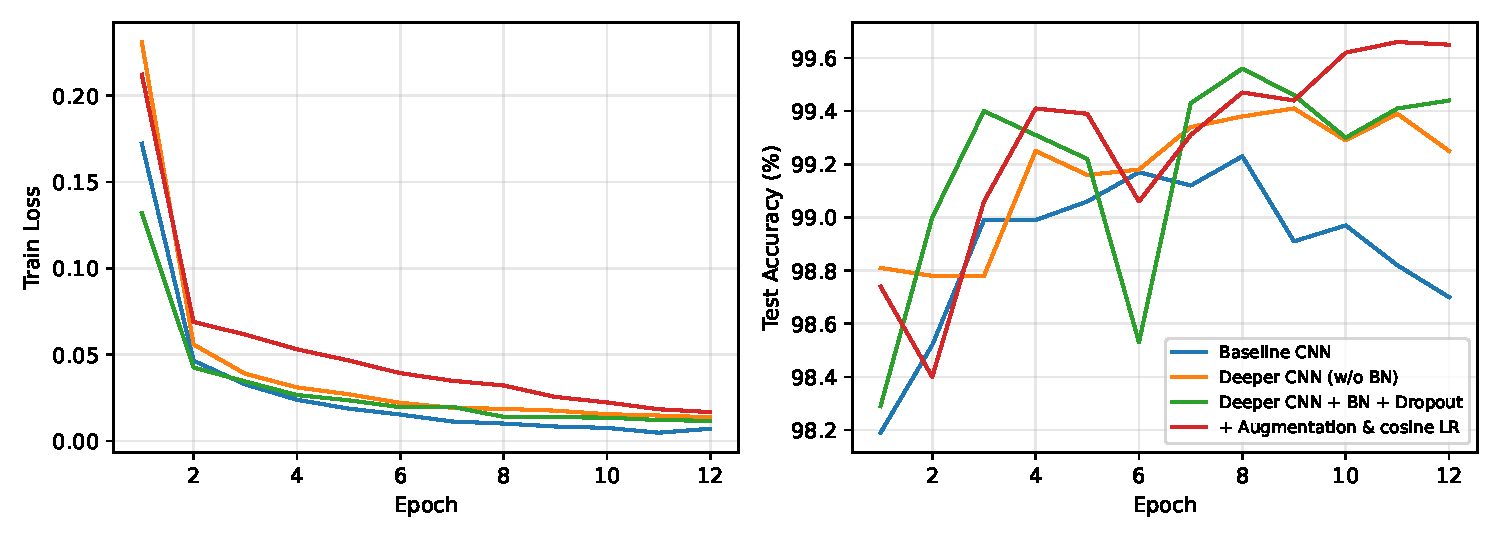
\includegraphics[width=\textwidth]{figures/training_curves.pdf}
  \caption{各实验训练损失（左）与测试准确率（右）曲线}
  \label{fig:curves}
\end{figure}

\begin{figure}[H]
  \centering
  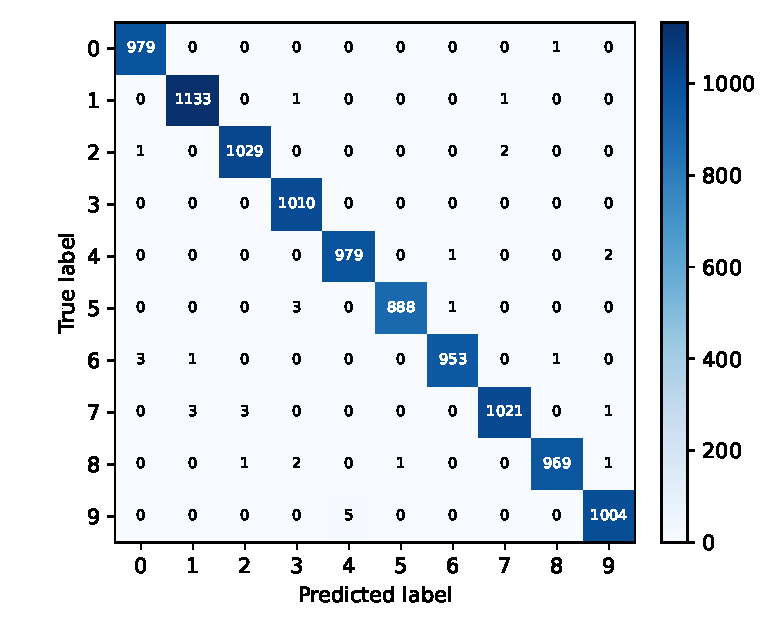
\includegraphics[width=0.62\textwidth]{figures/confusion_matrix.pdf}
  \caption{完整改进模型的测试集混淆矩阵（仅 34/10000 个样本分类错误）}
  \label{fig:cm}
\end{figure}

\mlConclusion{2}
结果分析如下：
\begin{enumerate}
  \item 加深网络（无 BN）将最优准确率由 99.23\% 提升至 99.41\%，说明更强的特征提取能力有效；
  \item 加入 BN 与 Dropout 后进一步提升至 99.56\%，且从图~\ref{fig:curves} 可见 BN 版本收敛更快、测试曲线更平滑，最终准确率也更稳定（99.44\% vs.\ 99.25\%）；
  \item 数据增强与余弦学习率虽然使训练变慢（每 epoch 样本需在线变换），但有效提升了泛化性能，最终得到 99.66\% 的最高准确率，且最优与最终准确率基本一致，过拟合被显著抑制；
  \item 混淆矩阵显示错误主要集中在易混数字对（如 4$\to$9、5$\to$3、7$\to$2），整体错误仅 34 个样本（0.34\%），性能已接近 MNIST 的人类水平。
\end{enumerate}

\section{总结}
本次作业从零设计并实现了基于 MNIST 的卷积神经网络，完成了 baseline 与改进模型的训练与对比分析。主要结论：(1) CNN 在 MNIST 上可达约 99\% 的准确率；(2) 加深网络、加入 BN/Dropout、数据增强与余弦学习率可逐级提升性能并抑制过拟合，最终模型测试准确率达到 99.66\%；(3) 各组件的消融对比验证了 BN 对收敛速度与稳定性的作用以及数据增强对泛化能力的作用。后续可以尝试 ResNet 风格的残差连接、更多 epoch 以及集成/蒸馏等方法进一步降低错误率；也可以迁移到 ImageNet-mini 等更复杂的数据集上验证结构的普适性。

\end{document}
